\documentclass{article}

% \usepackage{standalone}
 \usepackage{graphicx}
% \usepackage{media9}
%\graphicspath{{./images/}}
% \usepackage{amsmath}
\usepackage{multicol}
\usepackage{hyperref}
% \usepackage{setspace}                       \usepackage{geometry}          
%  \usepackage{longtable}                      
% \usepackage{chicago}                  
% \usepackage{times} 
% \usepackage{paracol}   % parallel columns    
% \usepackage[dvipsnames]{xcolor}       \usepackage{calc}                                      

% \usepackage{tikz}
% \usetikzlibrary{positioning, shadows, arrows, automata, shapes, calc, decorations.pathreplacing,calligraphy}

\title{Notes on Experiments}
\begin{document}
\maketitle
\tableofcontents \newpage
BASELINE PARAMETERS
\begin{verbatim}

        # LABOUR MARKET AND FIRM PARAMETERS
            'subsistence_wage': 40000., # psi
            'init_city_extent': 10.,    # CUT OR CHANGE?
            'seed_population': 400,
            'init_wage_premium_ratio': 0.2, # 1.2, ###

            # PARAMETERS MOST LIKELY TO AFFECT SCALE
            'c': 300                             ### .0,                            ###
            'price_of_output': 10,                 ######
            'density':600,                         #####
            'A': 3000,
            'alpha': 0.18,
            'beta':  0.75,
            'gamma': 0.12, ### reduced from .14
            'overhead': 1.5,
            'mult': 1.2,
            'adjN': 0.15,
            'adjk': 0.10,
            'adjn': 0.15,
            'adjF': 0.02,
            'adjw': 0.05, 
            'dist': 1, 
            'init_F': 100.0,
            'init_k': 500.0,
            'init_n': 100.0,

            # HOUSING AND MORTGAGE MARKET PARAMETERS
            'mortgage_period': 5.0,       # T, in years
            'working_periods': 40,        # in years
            'savings_rate': 0.3,
            'discount_rate': 0.07,        # 1/delta    Check THIS
            'r_prime': 0.05,
            'r_margin': 0.01,
            'property_tax_rate': 0.04,     # tau, annual rate, was c
            'housing_services_share': 0.3, # a
            'maintenance_share': 0.2,      # b
            'max_mortgage_share': 0.9,
            'ability_to_carry_mortgage': 0.28,
            'wealth_sensitivity': 0.1,
            'capital_gains_tax_person':   0.0, # share 0-1
            'capital_gains_tax_investor': 1, # share 0-1
    
\end{verbatim}
\newpage


\section{12-15 -010050 Change wealth sensitivity two cases 0.1 and 0.05 }
no sensitivity in any output for this parameter base. Ownership share may show  a small effect if we are near a tipping point driven by p-dot

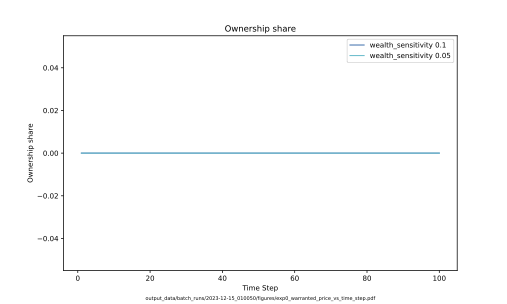
\includegraphics[scale=.45]{fig/Analysis/exp0_warranted_price_vs_time_step.png}


\begin{multicols}{2}
[\textbf{parameters}]
\begin{verbatim}
'adjn': 0.15,
'adjF': 0.02,
'adjw': 0.05, 
'capital_gains_tax_person':   0.0,
'capital_gains_tax_investor': 1,
\end{verbatim}

\end{multicols}
%%%%%%%%%%%%%%%%%%%%%%%%%%%%%%%%%%%%%%%%%%%%%
\newpage
\section{Change adjF - the growth rate of number of firms }

\begin{multicols}{2}
\begin{tabular}{c|c}
  mpl   &  up\\
  n   &  dn\\
  N   &  up\\
  F   & up \\
  E   &  up\\
  k   & dn
\end{tabular}

  notice the way firm number and size reverse as the adjustment speed changes. This makes sense
  
\end{multicols}

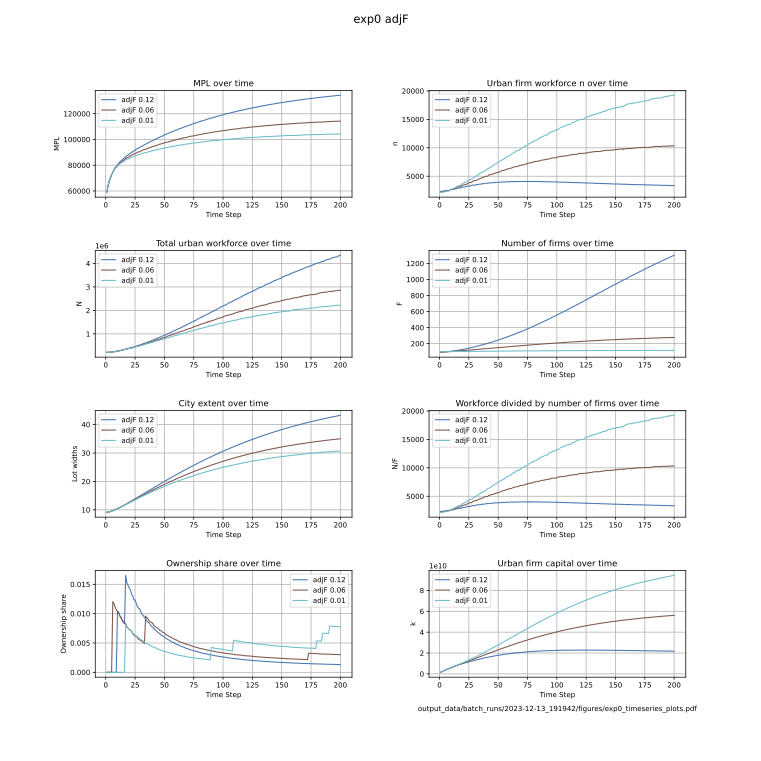
\includegraphics[scale=.55]{fig/Analysis/AdjF.png}

Notice too how MPL  is higher with a more rapid firm size adjustment. It keeps  firm workforce size down and pushes up MPL down, 

  Interestingly, city size is larger with faster growth of firm numbers. this is likely because with more firms hiring the population of the city grows faster.

%%%%%%%%%%%%%%%%%%%%%%%%%%%%%%%%%%%%%%%%%%%%%
\newpage
% \subsection{parameters}
% \begin{verbatim}

% \end{verbatim}

 \section{x12-15 010050, Change  Both adjF and adjn}
\begin{multicols}{2}
\begin{tabular}{c|c}
  mpl  &  \\
  n   &  \\
  N   &  \\
  F   &  \\
  E   &  \\
  k   & 
\end{tabular} 
Only three cases show (gold, turquoise, and purple). firm size and number show the same patternes as when just adF is changed 
\end{multicols}
% \begin{tabular}{l|c||c|c}
% parameters&&impact&\\ \hline
% & &  mpl  &  \\
% & &    n   &  \\
% & &    N   &  \\
% & & F   &  \\ 
% & &    Extent   &  \\
% & &    k   & 
% \end{tabular} 

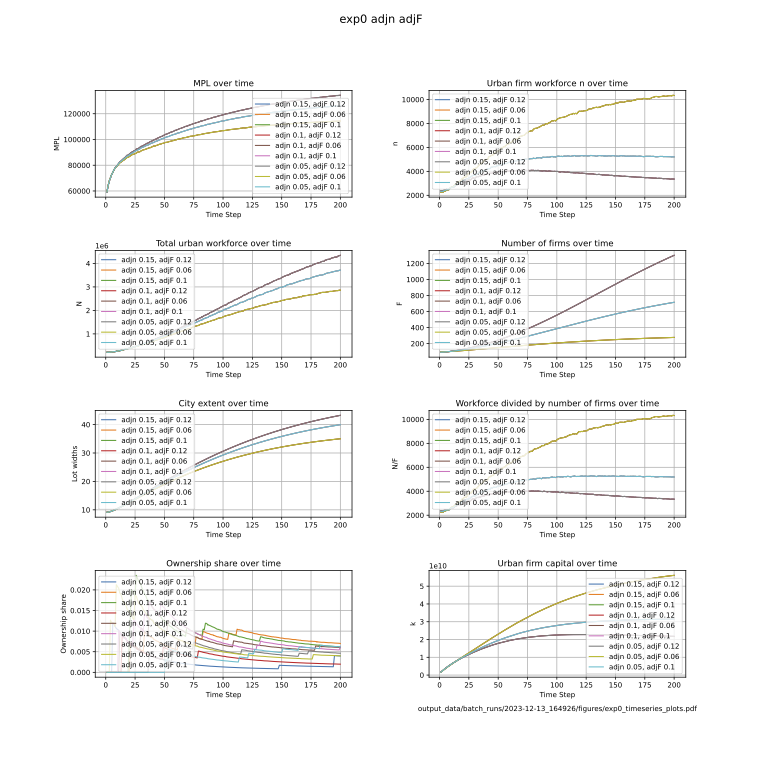
\includegraphics[scale=.55]{fig/Analysis/F-n-adjustment-speed.png}

% Subsistance wage typical 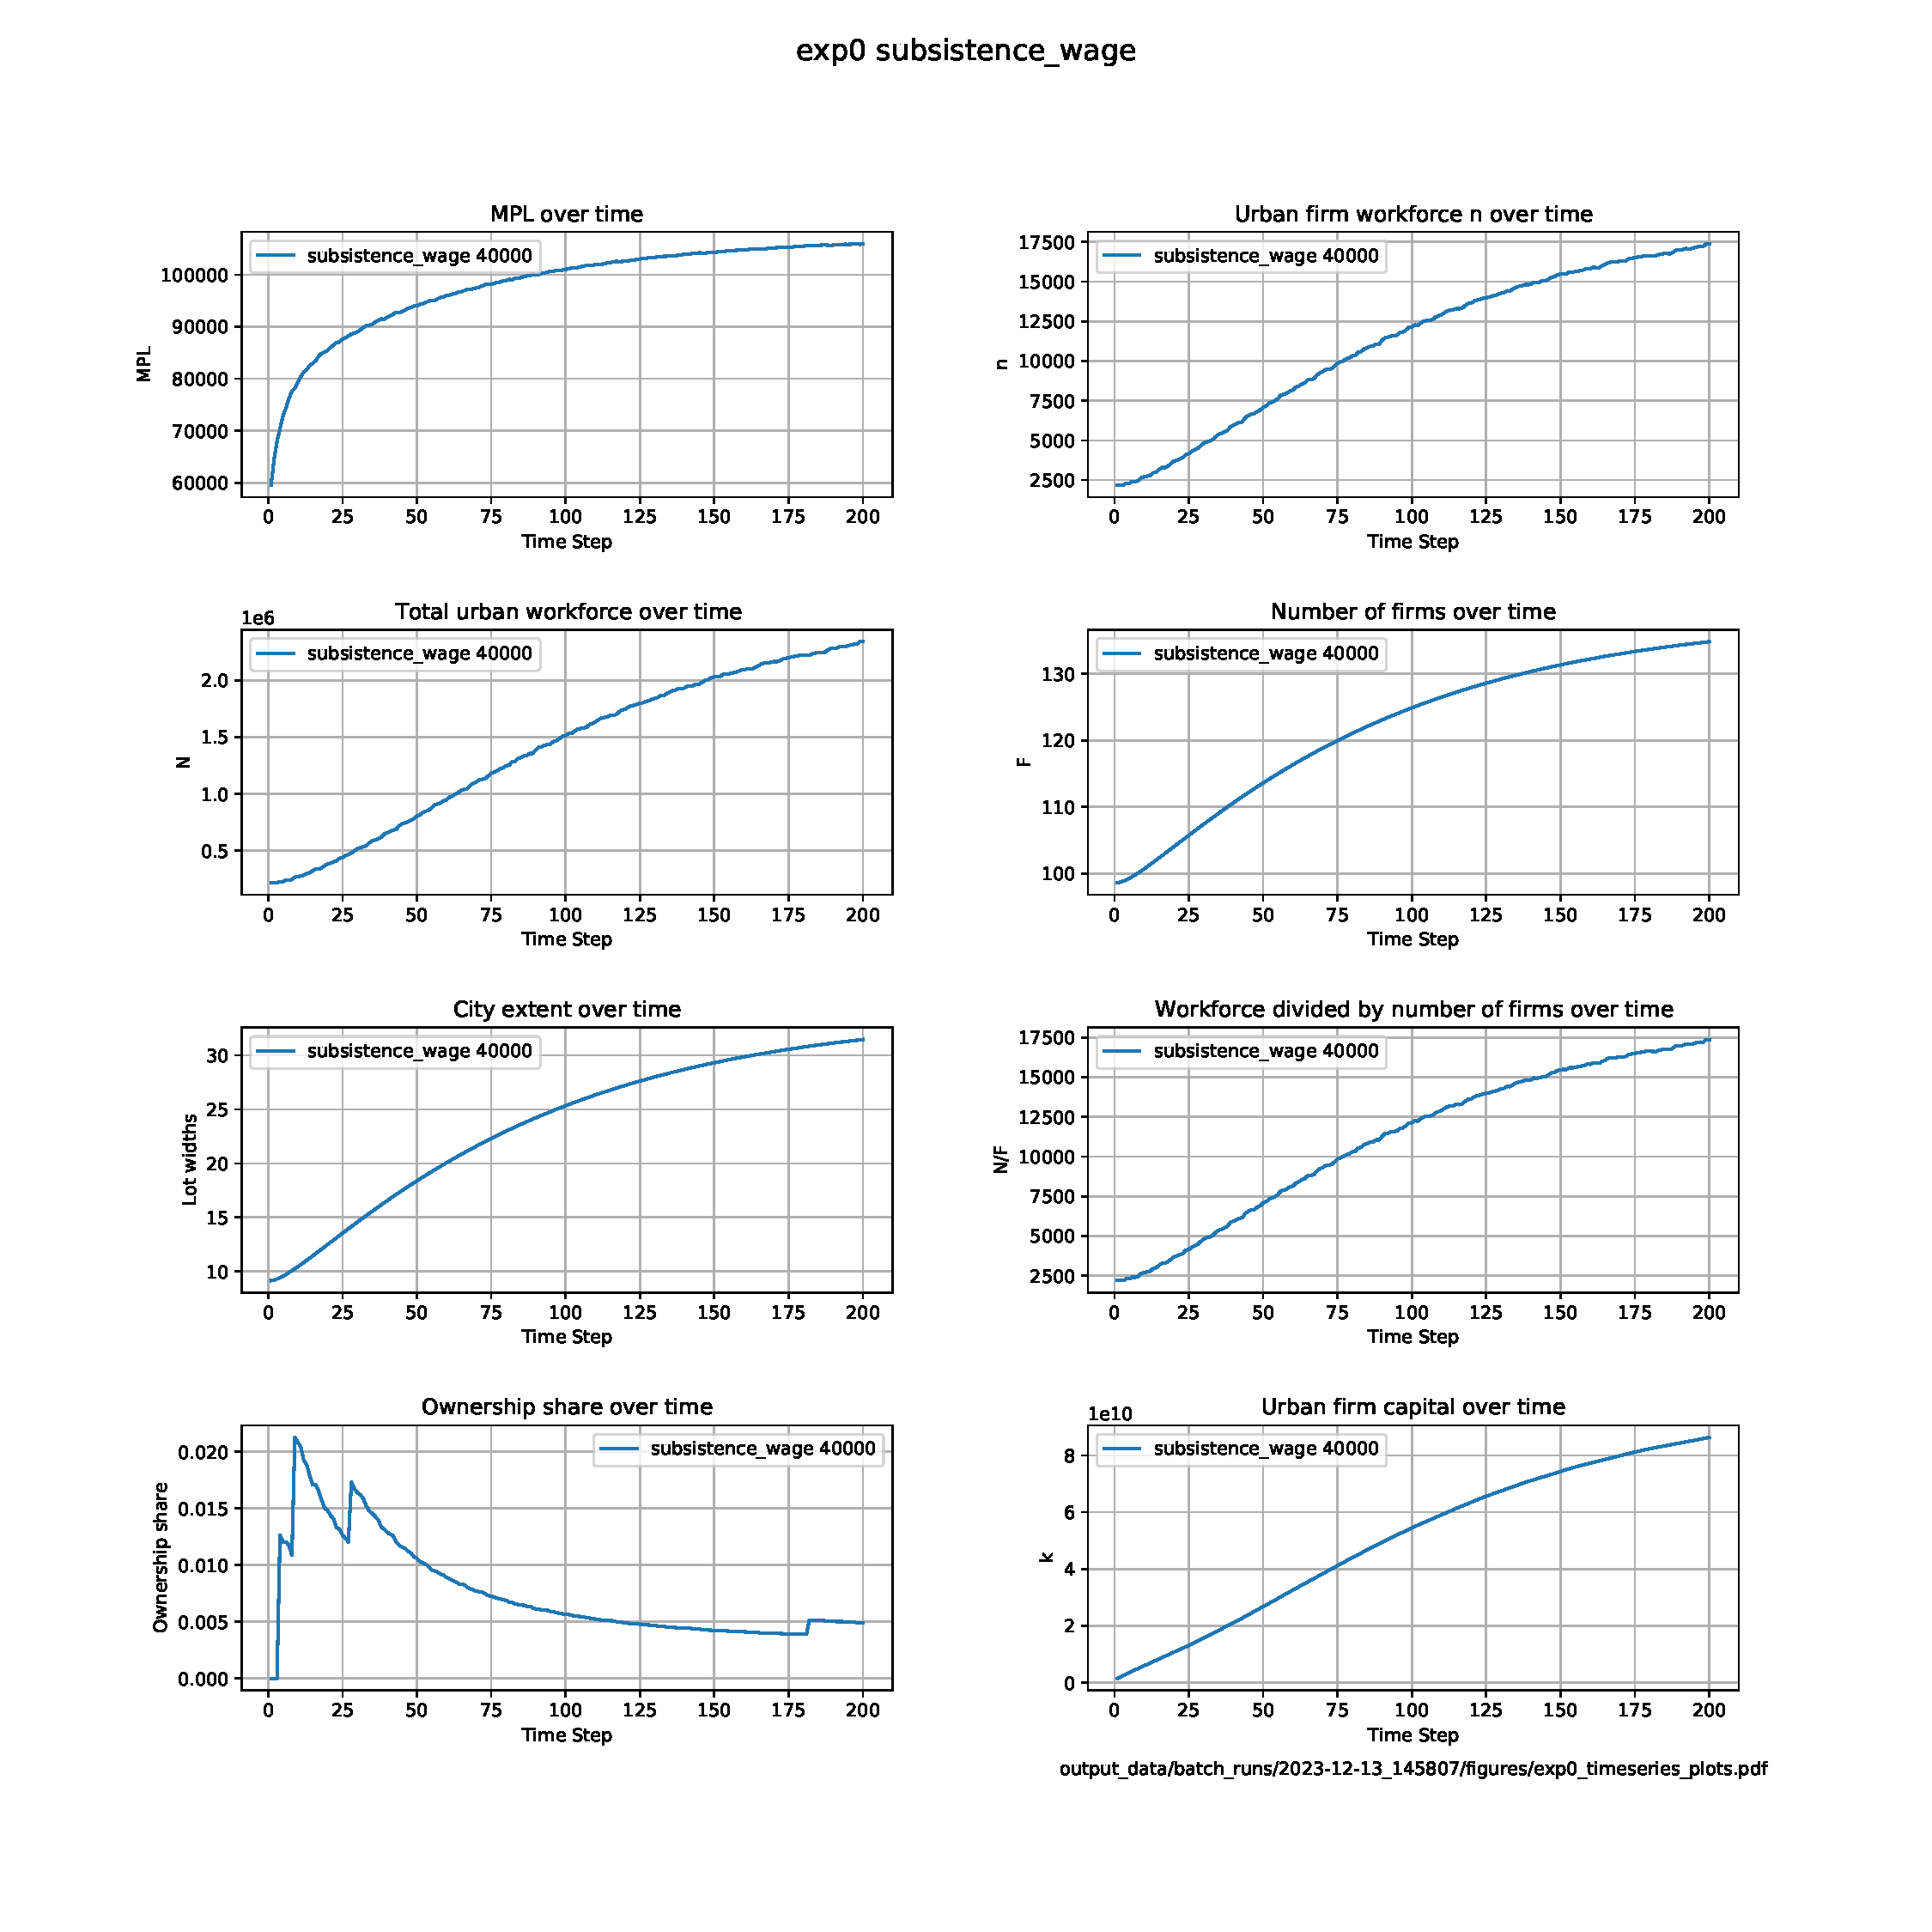
\includegraphics[scale=.55]{fig/Analysis/exp0-timeseries-plots.pdf}


We will want something like this perhaps in an early chapter. this case may not be interesting.
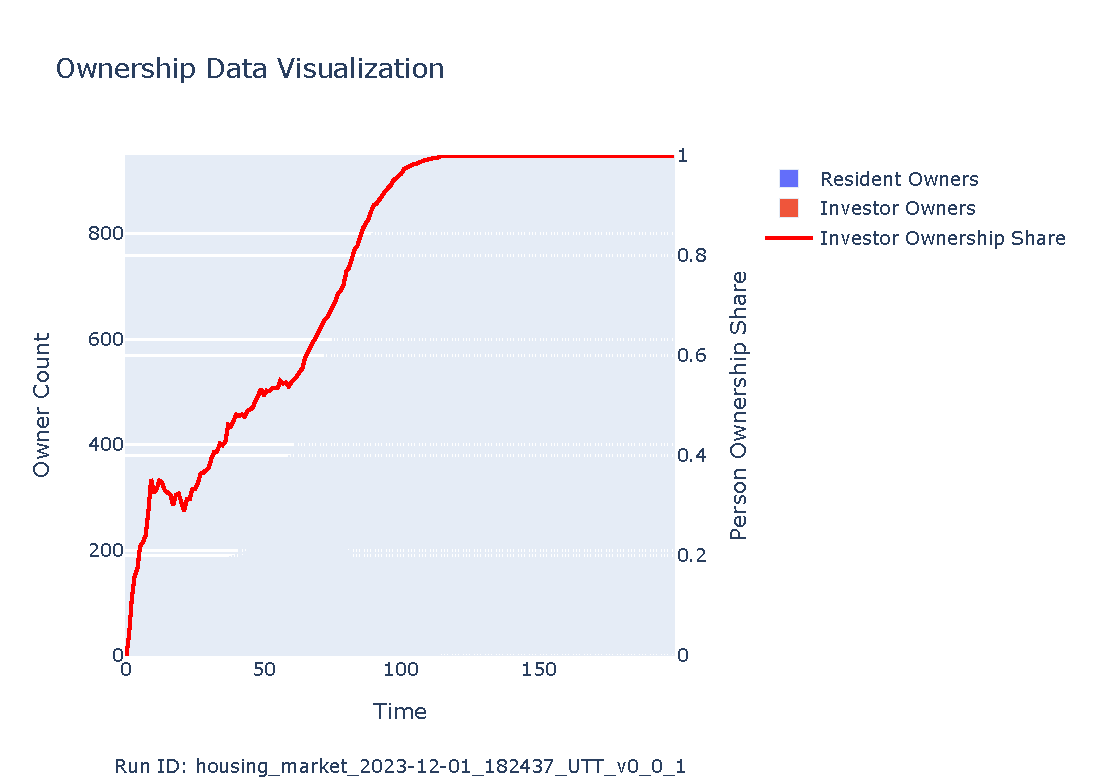
\includegraphics[scale=.95]{fig/Analysis/Ownership_Data_1.pdf}
% \subsection{parameters}
% \begin{verbatim}

% \end{verbatim}
\newpage
% \subsection{parameters}
% \begin{verbatim}

% \end{verbatim}

%%%%%%%%%%%%%%%%%%%%%%%%%%%%%%%%%%%%%%%%%%%%
 \section{12-17 010050, Varying Capital gains  }
\begin{tabular}{c|c}
  mpl  &  \\
  n   &  \\
  N   &  \\
  F   &  \\
  E   &  \\
  k   & 
\end{tabular} 

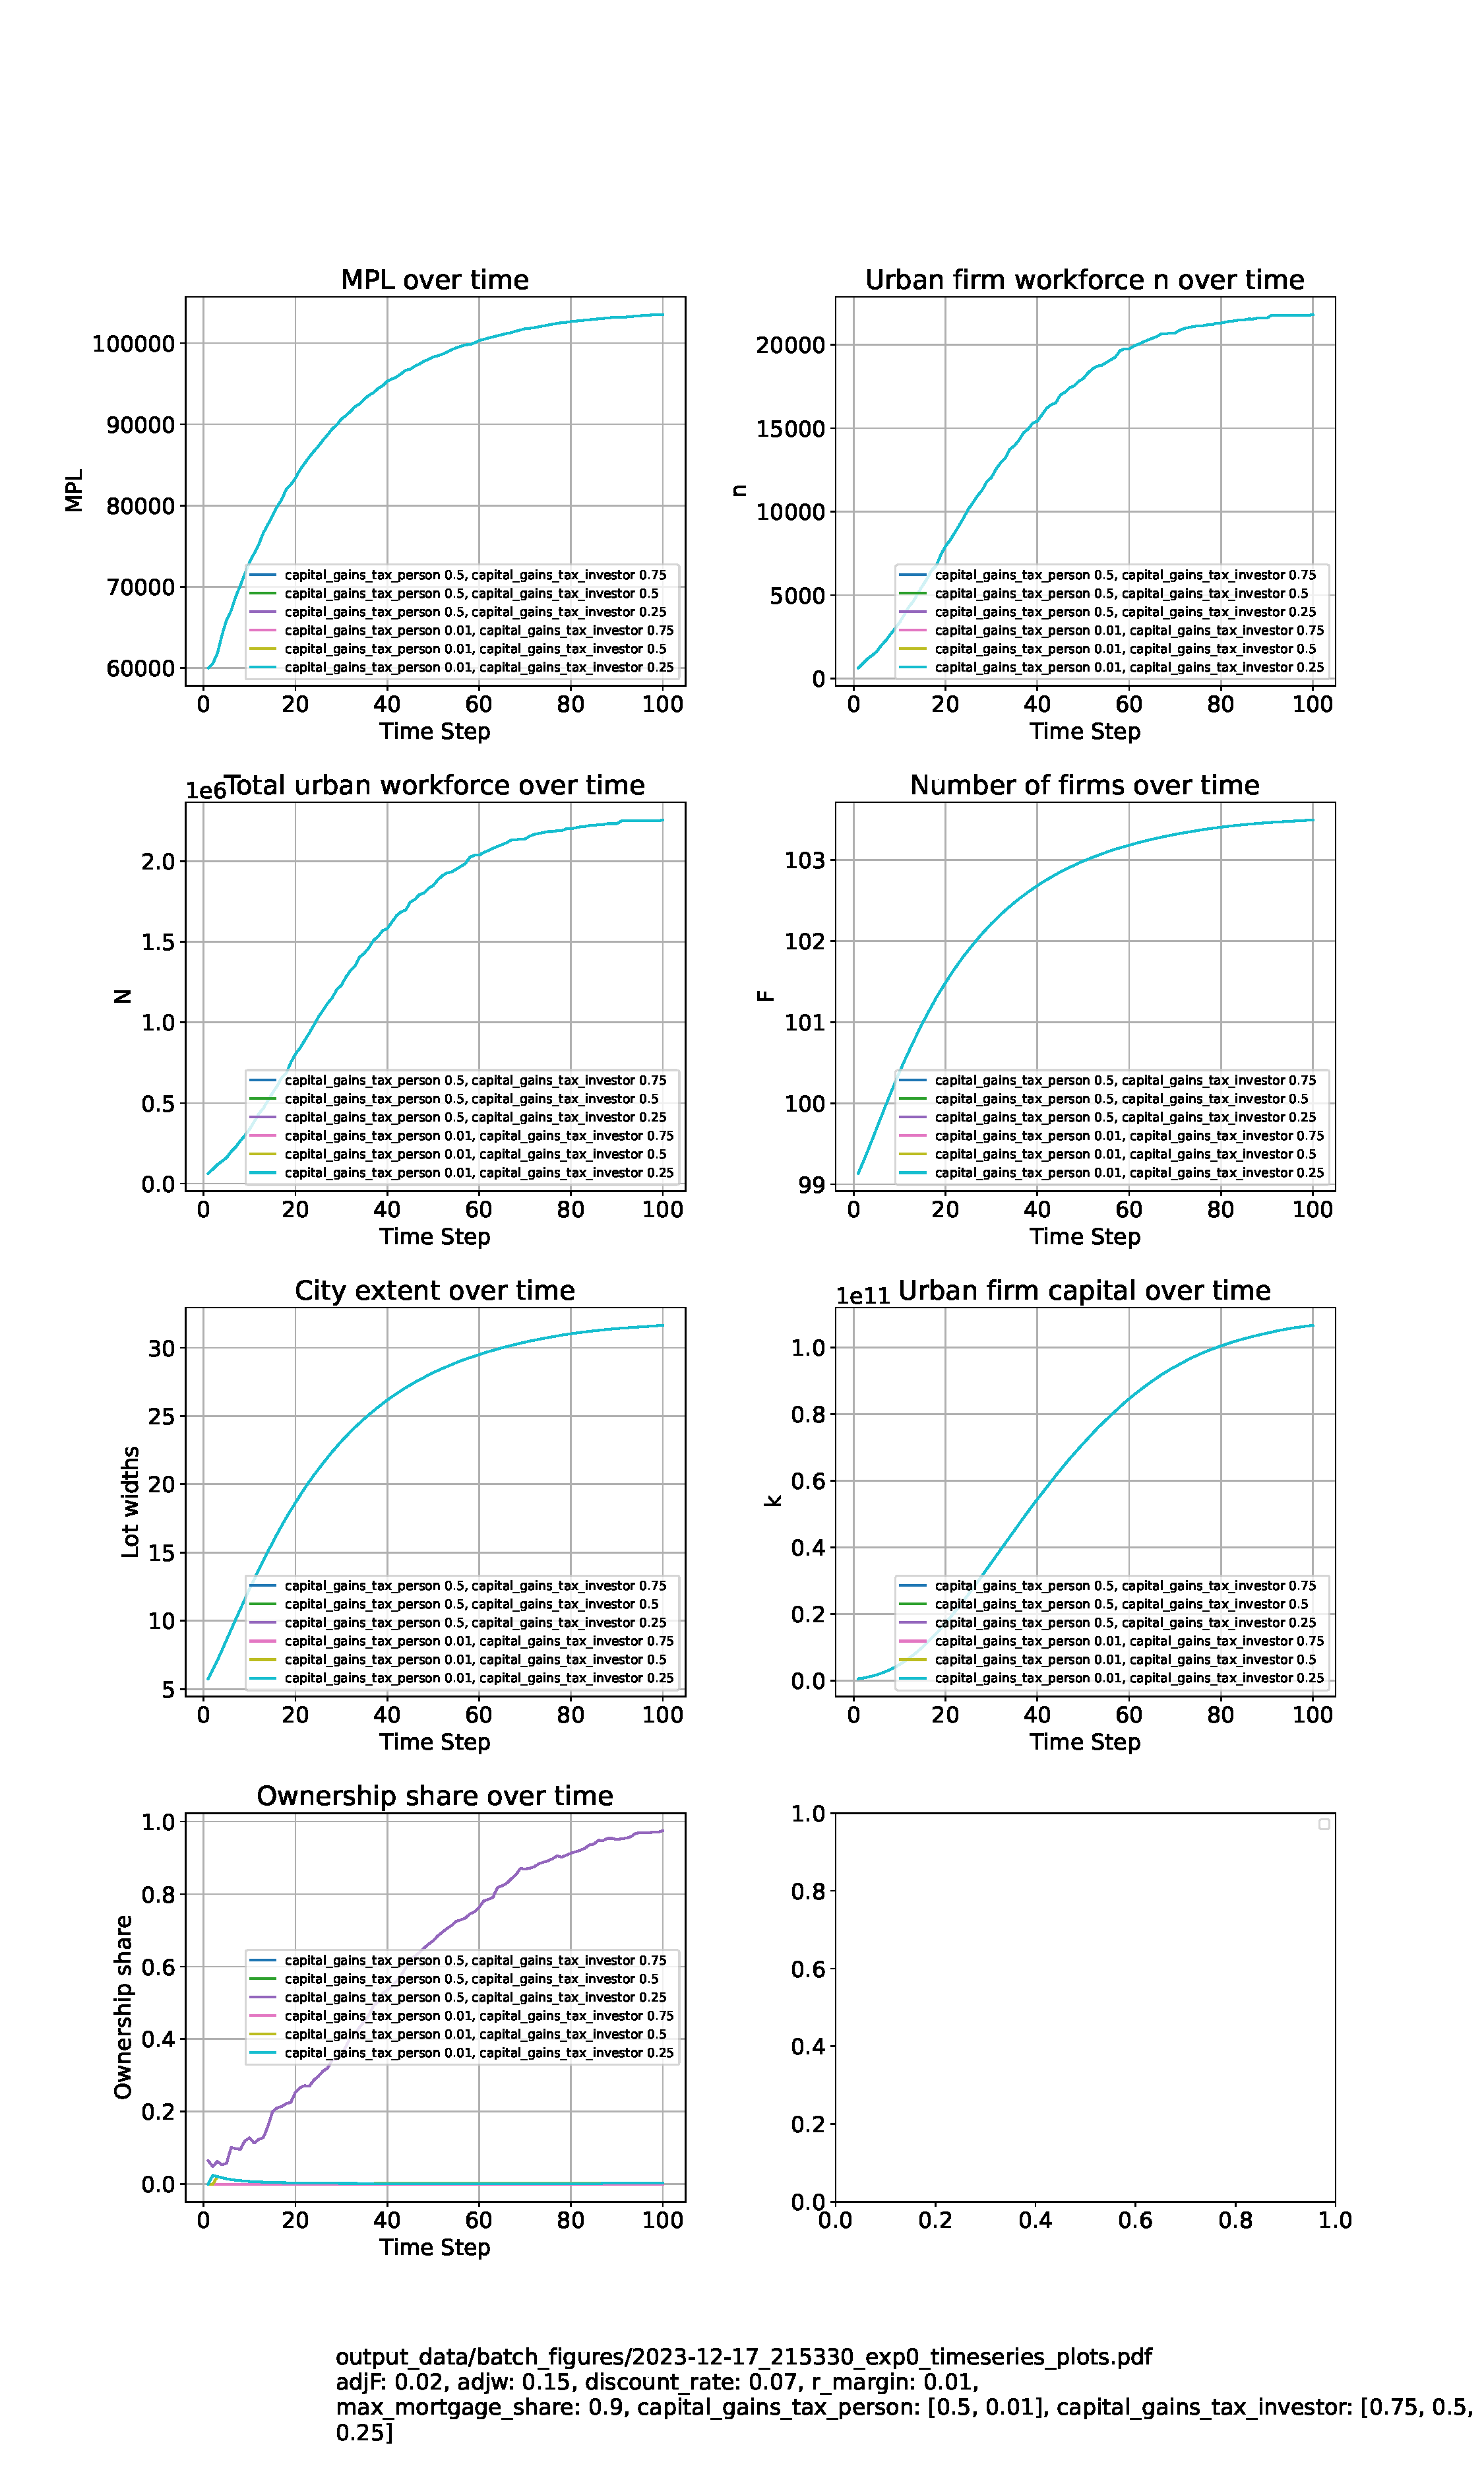
\includegraphics[trim= 1.5cm 5cm 2cm 6.5cm, clip, scale=.45]{fig/Analysis/215330-exp0-timeseries-plots.pdf}

% adjF: 0.02, adjw: 0.15, discount_rate: 0.07, r_margin: 0.01, max_mortgage_share: 0.9,  capital_gains_tax_person: [0.5, 0.01], capital_gains_tax_investor: [0.75, 0.5, 0.25

 \includegraphics[scale=.45, trim=2cm  5cm 2cm 4cm, clip]{fig/Analysis/2023-12-17_215330_exp0_timeseries_plots.pdf}

 \end{document}

 \newpage
% \subsection{parameters}
% \begin{verbatim}

% \end{verbatim}

% \section{Change  12-15 010050}
\begin{tabular}{c|c}
  mpl  &  \\
  n   &  \\
  N   &  \\
  F   &  \\
  E   &  \\
  k   & 
\end{tabular} 

% \includegraphics[scale=.25]{}
